\section{Help}

% \subsection{Table}
\begin{table}
	\begin{tabularx}{\textwidth}{XXXX}
		\toprule
		table & a & b \\
		\midrule
    $\alpha$ & 1 & 2 \\
    $\beta$  & 2 & 3 \\
    $\gamma$ & 3 & 4 \\
		\bottomrule
	\end{tabularx}
	\caption
	{
		\label{tab:example}
    table's label
	}
\end{table}

\subsection{Formula}

\begin{align}
	a_t & = \arg\max\limits_{a}\left(Q(s,a)+u(s,a)\right)\\
	Q(s,a) & =\frac{\bar{L}}{L(s,a)/N(s,a)} \\
	u(s,a) & = C_pP(s,a)\frac{\sqrt{\sum_bN(s,b)}}{1+N(s,a)}
\label{eqn:select}
\end{align}

% \subsection{Figure}
\begin{figure}
\centering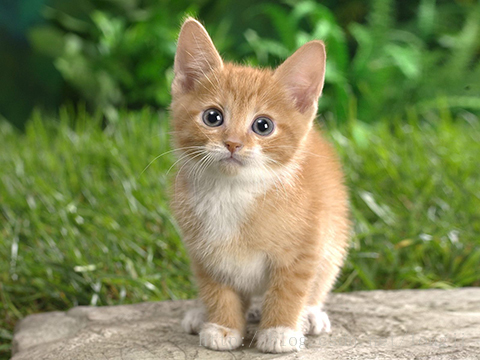
\includegraphics[height=0.36\textheight]{images/cat.jpeg}
\caption{
\label{fig:cat}
cute cat
}
\end{figure}

\subsection{Cite}
\begin{itemize}
\item \emph{References}: \cite{silver2017mastering}
\item \emph{Formula}: \ref{eqn:select}
\item \emph{Table}: \ref{tab:example}
\item \emph{Figure}: \ref{fig:cat}
\end{itemize}

\begin{enumerate}
\item \emph{Selection}: ...
\item \emph{Expansion}: ...
\item \emph{Simulation}: ...
\item \emph{Backpropagation}: ...
\end{enumerate}

\subsection*{No no. section}
